\section{Empirical Evaluation}
\label{sec:evaluation}

\subsection{Experimental Setup}

\paragraph{Algorithms}

We implemented the Spectral Experts algorithm using a proximal
subgradient descent algorithm\citationneeded for the low rank recovery
of $M_2$ and $M_3$. The algorithm was initialized with the regularized
least squares solution and was run to convergence in each instance. Both
regularization parameters were annealed as $\frac{1}{\sqrt{T}}$. 

We also implemented EM for this problem. In one set of experiments, we
initialized the parameters $\beta$ with random Gaussian entries with
mean zero and variance 1 and the mixture probabilities $\pi$ were
initialized to be uniform. We also compared the performance of EM when
initialized with the starting points given by Spectral Experts. We ran
EM for at most 1000 iterations, but in practice the experiments always
converged before this.

\paragraph{Datasets}

We ran our experiments on synthetically generated non-linear data. To
conform to the identifiability criteria discussed in
\sectionref{sec:algo}, we considered only features that would guarantee
this condition.

\begin{figure*}[t]
  \centering
  \subfigure{}{
    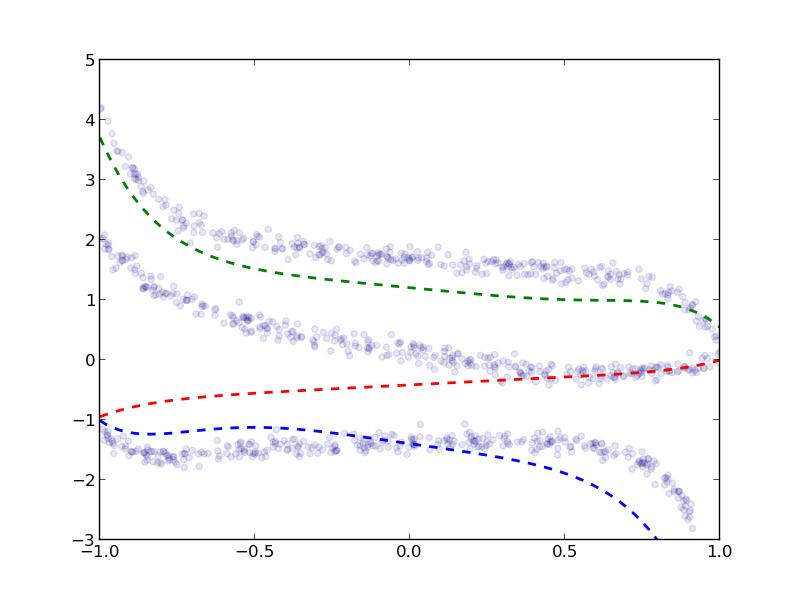
\includegraphics[width=0.30\textwidth]{figures/curves-vis/1-8-3-spec.png}}
  \subfigure{}{
    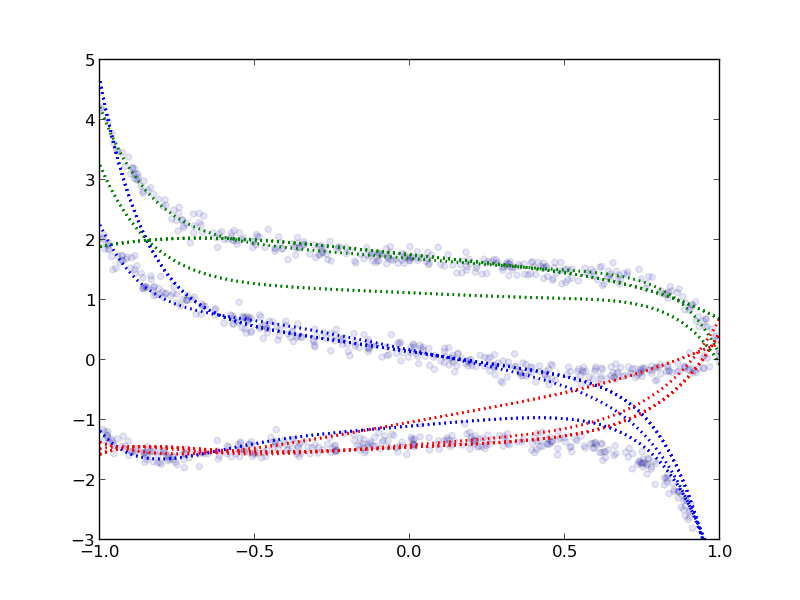
\includegraphics[width=0.30\textwidth]{figures/curves-vis/1-8-3-em.png}}
  \subfigure{}{
    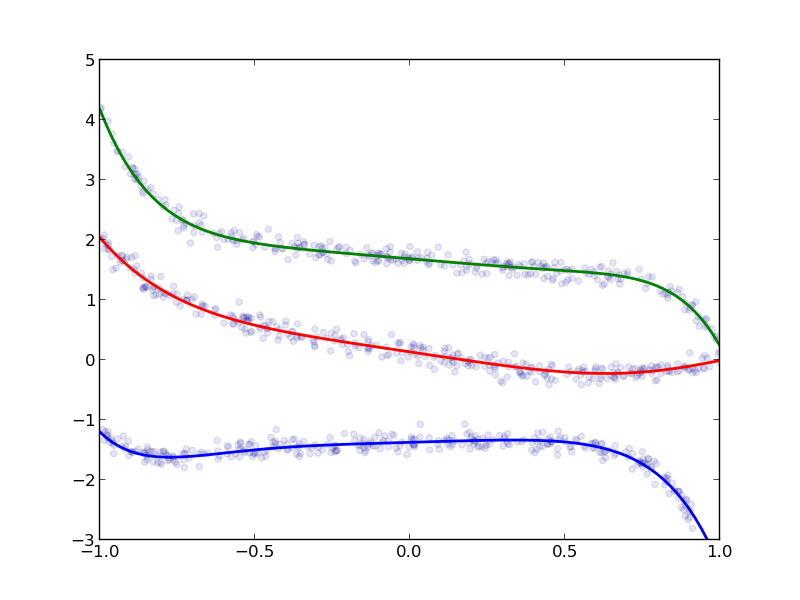
\includegraphics[width=0.30\textwidth]{figures/curves-vis/1-8-3-spem.png}}
  \label{fig:curves}
\end{figure*}

As an example, in the one dimensional scenario, one set of features we
considered were $\{1, x, x^4, x^7\}$. The data and the curves fit using
the spectral algorithm, EM with random initializations and EM
initialized with the parameters recovered using spectral experts are
plotted in \figureref{fig:curves}.

We generated $x$ uniformly from the unit hypercube.

Describe the Curves dataset.
$x = (1, t, t^4, t^9)$
$d = b^p$

Distribution over $x$.

Canonical settings:

Default values:
$n = 10^5$
$k = 5$

Dataset 1: visualization ($b = 1, p = 3$) 
Plot for visualization

Table on different settings: 
  (To show that we work comparably or better to EM always)
  (Spawned!)

Dataset 2: $b = 30$, $p = 1$
(Spawned many tasks to find spec performance. Will run EM on interesting cases)


\paragraph{Motion tracking data?}

\subsection{Results}

\paragraph{Basic results}

Punchline: spectral by itself is medicore, offers a good initialization to EM.
EM with random initialization is much less stable. (by table)

Using canonical settings, on the various datasets

Plot the parameters: the curves, three algorithms (DONE)

Plot: the histogram over errors (for EM?)

\paragraph{Effect on number of data points}

Curves dataset 2.
Plot: $n$ versus error for various algorithms

Point: tradeoff between statistical error and computational error;
not enough data, spectral is actually a lot worse
given enough data, spectral+EM is much better

\paragraph{Effect of dimensionality}

\paragraph{Effect of noise}

\paragraph{Effect of separation between components}
